\documentclass[12pt,a4paper]{article}

% Margins.
\setlength{\oddsidemargin}{0in}
\setlength{\evensidemargin}{0in}
\setlength{\headheight}{12pt}
\setlength{\headsep}{42pt}
\setlength{\topmargin}{-54pt}
\setlength{\textwidth}{6.5in}
\setlength{\textheight}{10in}

\usepackage{amsmath}
\usepackage{float}
\usepackage{graphicx}
\usepackage[hyphens]{url}
\usepackage{hyperref}	% Clickable links to figures, references and urls.

% Drawing.
\usepackage{pgf}
\usepackage{tikz}

% Listings for formatting code.
\usepackage{listings}
\usepackage{textcomp}
% General options.
\lstset{breaklines=true, basicstyle=\small\ttfamily, tabsize=4, numbers=left, stepnumber=1, frame=single, showstringspaces=false, upquote=true}
% C++ specific high-lighting. Comments are 50/50 shades of green/black and strings coloured with 60/40 red/black mixture.
\lstset{language=[ISO]C++, commentstyle=\color{green!50!black}, keywordstyle=\color{blue}, stringstyle=\color{red!60!black}}

%opening
\title{\vspace{-2cm}Programming for Engineers I\\Class 20\\Pointers, Arrays and Functions\\Passing By Reference}
\author{Attique Dawood}

\begin{document}
\maketitle
\section{Announcements}
\begin{itemize}
\item None.
\end{itemize}
\section{Revision}
\begin{itemize}
\item Pointers.
\item Passing arguments to functions.
\end{itemize}
\section{Pointers and Arrays}
The name of array is the pointer to its first element. A subscript besides array name can be translated in english as, ``access element located this much distance from start.'' Keep in mind that \verb|Array[i]| is the same as \verb|*(Array+i)| which means that you only need array pointer to access array elements using the subscript. Consider the following code
\begin{lstlisting}[caption={Arrays and Pointers}]
#include <iostream>
using namespace std;

int Area(int*, int*); // Function prototype.

int main()
{
	int Array[5] = {3,7,2,1,5};

	cout << Array << endl; // Prints the address of array.

	// Using subscript.
	cout << Array[0] << endl; // Print the value of element located a distance of 0 from start.
	cout << Array[3] << endl; // Print the value of element located a distance of 3 from start.
	cout << Array[5] << endl; // Print the value of element located a distance of 5 from start. ERROR! Out of bound.

	// Using Pointers.
	cout << *(Array+0) << endl; // Prints the value of first element which is 3.
	cout << *(Array+1) << endl; // Prints the value of second element which is 7.
	cout << *(Array+5) << endl; // Prints the value of sixth element which out of bound or ERROR.

	return 0;
}
\end{lstlisting}
\begin{figure}[H]
\centering
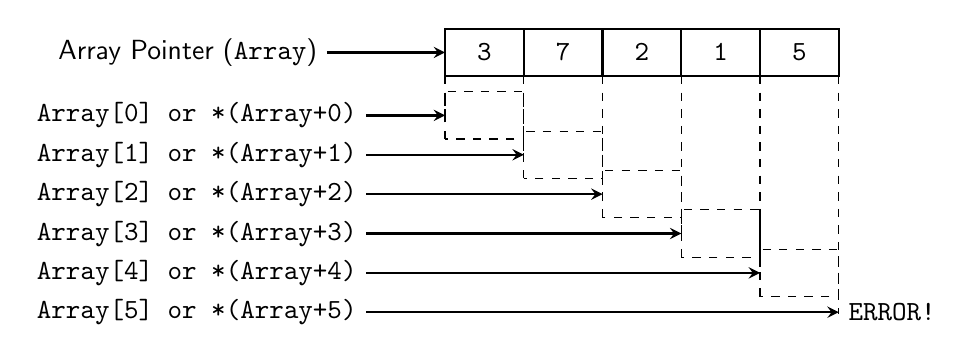
\begin{tikzpicture}
	% Writing 'Array'
	\coordinate [label=left:\textsf{Array Pointer (\texttt{Array})}] (Arraypointer) at (-1.5cm,0.3cm);
	\draw[thick, ->, >=stealth] (-1.5cm, 0.3cm) -- (0cm, 0.3cm);
	% Drawing boxes.
	\foreach \x in {0.0cm, 1.0cm, 2.0cm, 3.0cm, 4.0cm}
		\draw[thick] (\x, 0cm) rectangle (\x+1.0cm, 0.6cm);
	% Writing numbers in boxes. This is original array.
	\foreach \x/\y in {0.0cm/3, 1.0cm/7, 2.0cm/2, 3.0cm/1, 4.0cm/5}
		\draw (\x+0.5cm,0.3cm) node {\texttt{\y}};
	\def\XD{0cm}
	\def\YD{-0.5cm}
	% Drawing an arrow and pointer.
	\coordinate [label=left:\texttt{Array[0] or *(Array+0)}] (Array0) at (-1cm,\YD);
	\draw[thick, ->, >=stealth] (-1cm, \YD) -- (0cm+\XD, \YD);
	\draw[dashed] (\XD,0cm) -- (\XD,\YD-0.5);
	\draw[dashed] (\XD,\YD-0.3cm) rectangle (\XD+1cm,\YD+0.3cm);

	\def\XD{1cm}
	\def\YD{-1cm}
	% Drawing an arrow and pointer.
	\coordinate [label=left:\texttt{Array[1] or *(Array+1)}] (Array1) at (-1cm,\YD);
	\draw[thick, ->, >=stealth] (-1cm, \YD) -- (0cm+\XD, \YD);
	\draw[dashed] (\XD,0cm) -- (\XD,\YD-0.5);
	\draw[dashed] (\XD,\YD-0.3cm) rectangle (\XD+1cm,\YD+0.3cm);

	\def\XD{2cm}
	\def\YD{-1.5cm}
	% Drawing an arrow and pointer.
	\coordinate [label=left:\texttt{Array[2] or *(Array+2)}] (Array2) at (-1cm,\YD);
	\draw[thick, ->, >=stealth] (-1cm, \YD) -- (0cm+\XD, \YD);
	\draw[dashed] (\XD,0cm) -- (\XD,\YD-0.5);
	\draw[dashed] (\XD,\YD-0.3cm) rectangle (\XD+1cm,\YD+0.3cm);

	\def\XD{3cm}
	\def\YD{-2cm}
	% Drawing an arrow and pointer.
	\coordinate [label=left:\texttt{Array[3] or *(Array+3)}] (Array3) at (-1cm,\YD);
	\draw[thick, ->, >=stealth] (-1cm, \YD) -- (0cm+\XD, \YD);
	\draw[dashed] (\XD,0cm) -- (\XD,\YD-0.5);
	\draw[dashed] (\XD,\YD-0.3cm) rectangle (\XD+1cm,\YD+0.3cm);
	
	\def\XD{4cm}
	\def\YD{-2.5cm}
	% Drawing an arrow and pointer.
	\coordinate [label=left:\texttt{Array[4] or *(Array+4)}] (Array4) at (-1cm,\YD);
	\draw[thick, ->, >=stealth] (-1cm, \YD) -- (0cm+\XD, \YD);
	\draw[dashed] (\XD,0cm) -- (\XD,\YD-0.5);
	\draw[dashed] (\XD,\YD-0.3cm) rectangle (\XD+1cm,\YD+0.3cm);
	
	\def\XD{5cm}
	\def\YD{-3cm}
	% Drawing an arrow and pointer.
	\coordinate [label=left:\texttt{Array[5] or *(Array+5)}] (Array5) at (-1cm,\YD);
	\draw[thick, ->, >=stealth] (-1cm, \YD) -- (0cm+\XD, \YD);
	\draw[dashed] (\XD,0cm) -- (\XD,\YD-0.5);
	\coordinate [label=right:\texttt{ERROR!}] (Error) at (\XD,\YD);
\end{tikzpicture}
\caption{Using pointer to access array elements}
\label{Array-pointer-element-access}
\end{figure}
\section{Passing By Value and By Reference}
\begin{itemize}
\item Basic data types are always passed by value to functions. A `local' copy of variable is created in function and used.
\item Extra variables created in function may take up sizeable memory if there are many input arguments. Large arrays if passed as copy can create problems.
\item Variables can be passed as reference by specifying a preceding \verb|&| with variable name. \textbf{There is no change in function call}.
\end{itemize}
\begin{lstlisting}[caption={Passing Function Arguments as Reference}]
//This function calculates the square of a number and returns it.
#include <iostream>
using namespace std;

int sum(int& A, int& B)
{
    int result = A+B;
    return result;
}

void main()
{
    int x = 3;
    int y = 7;
    
    cout << sum(x, y) << endl;
    
    return 0;
}
\end{lstlisting}
\section{Memory Map in a Normal Function Call}
Consider the code in listing 1. Before the function call on line 8 the memory will contain three variable a, b and c. Inside the function, three additional variables, x, y and z, will be created. Values of a and b will be copied into x and y as these are the function arguments. After the function call ends, value of z, which is 15, will be copied onto c. Variables x, y and z will be destroyed or deallocated after function call. Figure \ref{A-Normal-Function-Call} gives a picture of exactly how this happens.
\begin{lstlisting}[caption={Calling a function}]
#include <cstdio>
int Area(int, int); // Function prototype.
int main()
{
	int a, b, c;
	a = 3;
	b = 5;
	c = Area(a, b); // Function call.
	
	return 0;
}
// Function definition.
int Area(int x, int y)
{
	int z;
	z = x*y;
	return z;
}
\end{lstlisting}
\begin{figure}[H]
\centering
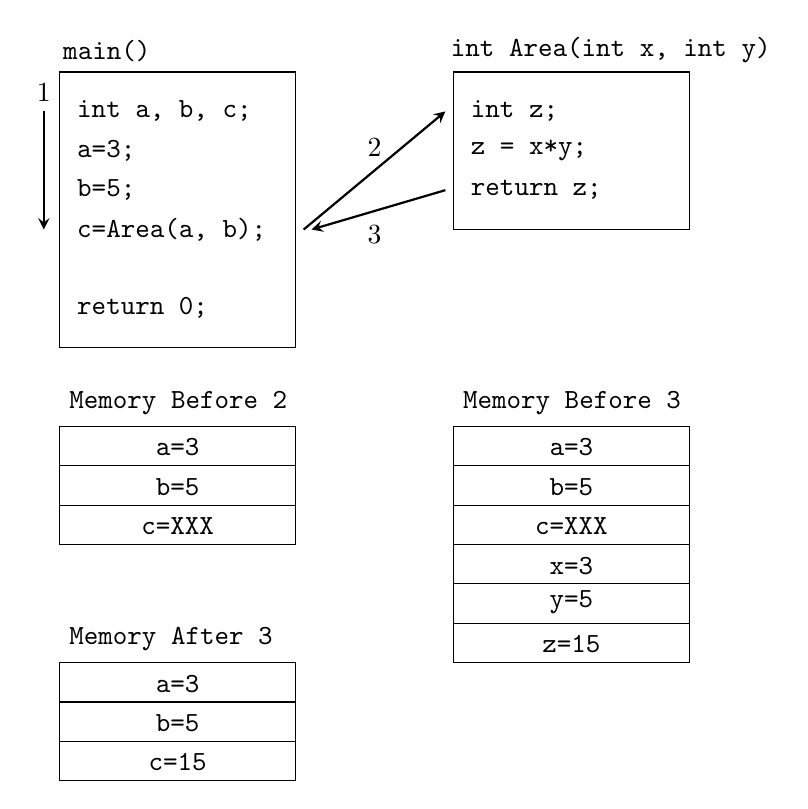
\begin{tikzpicture}
	% Drawing main()
	\coordinate [label=above:\texttt{main()}] (main) at (0.6cm,0cm);
	\draw (0cm,0cm) rectangle (3cm,-3.5cm);
	\coordinate [label=right:\texttt{int a, b, c;}] (intabc) at (0.1cm,-0.5cm);
	\coordinate [label=right:\texttt{a=3;}] (a3) at (0.1cm,-1cm);
	\coordinate [label=right:\texttt{b=5;}] (b5) at (0.1cm,-1.5cm);
	\coordinate [label=right:\texttt{c=Area(a, b);}] (carea) at (0.1cm,-2cm);
	\coordinate [label=right:\texttt{return 0;}] (return0) at (0.1cm,-3cm);

	% Drawing Area() function.
	\coordinate [label=above:\texttt{int Area(int x, int y)}] (main) at (7cm,0cm);
	\draw (5cm,0cm) rectangle (8cm,-2cm);
	\coordinate [label=right:\texttt{int z;}] (intz) at (5.1cm,-0.5cm);
	\coordinate [label=right:\texttt{z = x*y;}] (zxy) at (5.1cm,-1cm);
	\coordinate [label=right:\texttt{return z;}] (return z) at (5.1cm,-1.5cm);

	% Drawing arrows
	\coordinate [label=above:1] (1) at (-0.2cm,-0.5cm);
	\draw[thick, ->, >=stealth] (-0.2cm, -0.5cm) -- (-0.2cm, -2cm);
	\coordinate [label=above:2] (2) at (4cm,-1.2cm);
	\draw[thick, ->, >=stealth] (3.1cm, -2cm) -- (4.9cm, -0.5cm);
	\coordinate [label=above:3] (3) at (4cm,-2.3cm);
	\draw[thick, ->, >=stealth] (4.9cm, -1.5cm) -- (3.2cm, -2cm);
	
	% Drawing Memory Map.
	\coordinate [label=right:\texttt{Memory Before 2}] (Memory1) at (0cm,-4.2cm);
	\draw (0cm,-4.5cm) rectangle (3cm,-5cm);
	\coordinate [label=above:\texttt{a=3}] (a3) at (1.5cm,-5cm);
	\draw (0cm,-5cm) rectangle (3cm,-5.5cm);
	\coordinate [label=above:\texttt{b=5}] (b5) at (1.5cm,-5.5cm);
	\draw (0cm,-5.5cm) rectangle (3cm,-6cm);
	\coordinate [label=above:\texttt{c=XXX}] (cXXX) at (1.5cm,-6cm);
	
	\coordinate [label=right:\texttt{Memory Before 3}] (Memory2) at (5cm,-4.2cm);
	\draw (5cm,-4.5cm) rectangle (8cm,-5cm);
	\coordinate [label=above:\texttt{a=3}] (a3) at (6.5cm,-5cm);
	\draw (5cm,-5cm) rectangle (8cm,-5.5cm);
	\coordinate [label=above:\texttt{b=5}] (b5) at (6.5cm,-5.5cm);
	\draw (5cm,-5.5cm) rectangle (8cm,-6cm);
	\coordinate [label=above:\texttt{c=XXX}] (cXXX) at (6.5cm,-6cm);
	\draw (5cm,-6cm) rectangle (8cm,-6.5cm);
	\coordinate [label=above:\texttt{x=3}] (x3) at (6.5cm,-6.5cm);
	\draw (5cm,-6.5cm) rectangle (8cm,-7cm);
	\coordinate [label=above:\texttt{y=5}] (y5) at (6.5cm,-7cm);
	\draw (5cm,-5cm) rectangle (8cm,-7.5cm);
	\coordinate [label=above:\texttt{z=15}] (z15) at (6.5cm,-7.5cm);
	
	\coordinate [label=right:\texttt{Memory After 3}] (Memory3) at (0cm,-7.2cm);
	\draw (0cm,-7.5cm) rectangle (3cm,-8cm);
	\coordinate [label=above:\texttt{a=3}] (a3) at (1.5cm,-8cm);
	\draw (0cm,-8cm) rectangle (3cm,-8.5cm);
	\coordinate [label=above:\texttt{b=5}] (b5) at (1.5cm,-8.5cm);
	\draw (0cm,-8.5cm) rectangle (3cm,-9cm);
	\coordinate [label=above:\texttt{c=15}] (c15) at (1.5cm,-9cm);
\end{tikzpicture}
\caption{A normal function call}
\label{A-Normal-Function-Call}
\end{figure}
\section{Passing by Reference}
If function arguments are passed--by--reference then the function arguments directly refer to the original variables. New variables are not created. If the value of function arguments is changed then the value of original arguments is also varied. Syntax for passing variables by reference is giving in code listing 2.
\begin{lstlisting}[caption={Passing by reference}]
#include <cstdio>
int Area(int&, int&); // Function prototype.
int main()
{
	int a, b, c;
	a = 3;
	b = 5;
	c = Area(a, b); // Function call.
	
	return 0;
}
// Function definition.
int Area(int& x, int& y)
{
	int z = x*y;
	x=7;
	return z;
}
\end{lstlisting}
\begin{figure}[H]
\centering
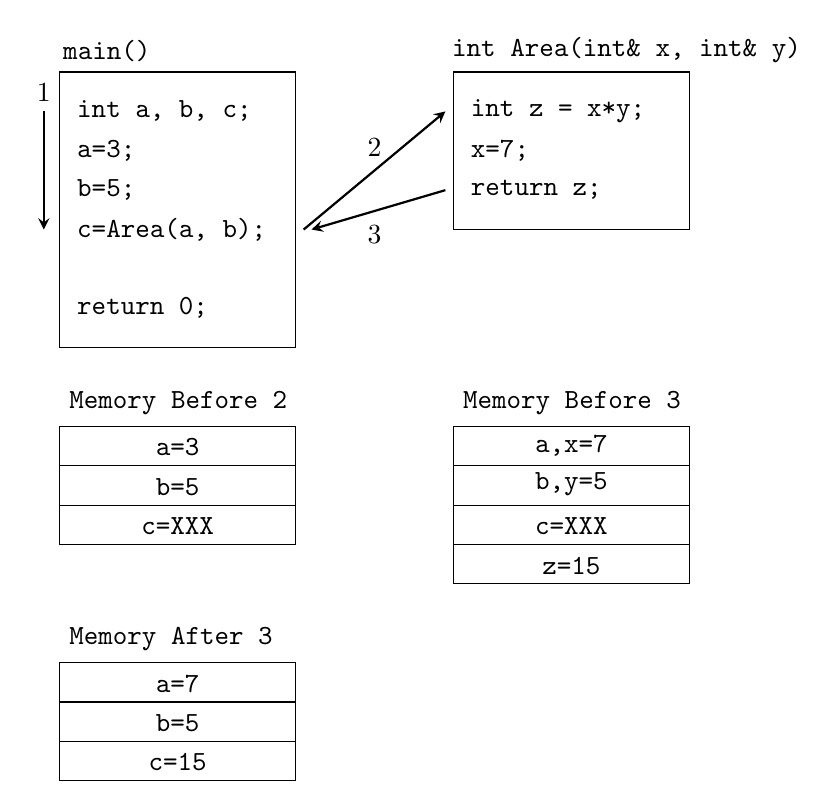
\begin{tikzpicture}
	% Drawing main()
	\coordinate [label=above:\texttt{main()}] (main) at (0.6cm,0cm);
	\draw (0cm,0cm) rectangle (3cm,-3.5cm);
	\coordinate [label=right:\texttt{int a, b, c;}] (intabc) at (0.1cm,-0.5cm);
	\coordinate [label=right:\texttt{a=3;}] (a3) at (0.1cm,-1cm);
	\coordinate [label=right:\texttt{b=5;}] (b5) at (0.1cm,-1.5cm);
	\coordinate [label=right:\texttt{c=Area(a, b);}] (carea) at (0.1cm,-2cm);
	\coordinate [label=right:\texttt{return 0;}] (return0) at (0.1cm,-3cm);

	% Drawing Area() function.
	\coordinate [label=above:\texttt{int Area(int\& x, int\& y)}] (main) at (7.2cm,0cm);
	\draw (5cm,0cm) rectangle (8cm,-2cm);
	\coordinate [label=right:\texttt{int z = x*y;}] (zxy) at (5.1cm,-0.5cm);
	\coordinate [label=right:\texttt{x=7;}] (x7) at (5.1cm,-1cm);
	\coordinate [label=right:\texttt{return z;}] (return z) at (5.1cm,-1.5cm);

	% Drawing arrows
	\coordinate [label=above:1] (1) at (-0.2cm,-0.5cm);
	\draw[thick, ->, >=stealth] (-0.2cm, -0.5cm) -- (-0.2cm, -2cm);
	\coordinate [label=above:2] (2) at (4cm,-1.2cm);
	\draw[thick, ->, >=stealth] (3.1cm, -2cm) -- (4.9cm, -0.5cm);
	\coordinate [label=above:3] (3) at (4cm,-2.3cm);
	\draw[thick, ->, >=stealth] (4.9cm, -1.5cm) -- (3.2cm, -2cm);
	
	% Drawing Memory Map.
	\coordinate [label=right:\texttt{Memory Before 2}] (Memory1) at (0cm,-4.2cm);
	\draw (0cm,-4.5cm) rectangle (3cm,-5cm);
	\coordinate [label=above:\texttt{a=3}] (a3) at (1.5cm,-5cm);
	\draw (0cm,-5cm) rectangle (3cm,-5.5cm);
	\coordinate [label=above:\texttt{b=5}] (b5) at (1.5cm,-5.5cm);
	\draw (0cm,-5.5cm) rectangle (3cm,-6cm);
	\coordinate [label=above:\texttt{c=XXX}] (cXXX) at (1.5cm,-6cm);
	
	\coordinate [label=right:\texttt{Memory Before 3}] (Memory2) at (5cm,-4.2cm);
	\draw (5cm,-4.5cm) rectangle (8cm,-5cm);
	\coordinate [label=above:\texttt{a,x=7}] (a3) at (6.5cm,-5cm);
	\draw (5cm,-5cm) rectangle (8cm,-5.5cm);
	\coordinate [label=above:\texttt{b,y=5}] (b5) at (6.5cm,-5.5cm);
	\draw (5cm,-5.5cm) rectangle (8cm,-6cm);
	\coordinate [label=above:\texttt{c=XXX}] (cXXX) at (6.5cm,-6cm);
	\draw (5cm,-6cm) rectangle (8cm,-6.5cm);
	\coordinate [label=above:\texttt{z=15}] (z15) at (6.5cm,-6.5cm);
	
	\coordinate [label=right:\texttt{Memory After 3}] (Memory3) at (0cm,-7.2cm);
	\draw (0cm,-7.5cm) rectangle (3cm,-8cm);
	\coordinate [label=above:\texttt{a=7}] (a3) at (1.5cm,-8cm);
	\draw (0cm,-8cm) rectangle (3cm,-8.5cm);
	\coordinate [label=above:\texttt{b=5}] (b5) at (1.5cm,-8.5cm);
	\draw (0cm,-8.5cm) rectangle (3cm,-9cm);
	\coordinate [label=above:\texttt{c=15}] (c15) at (1.5cm,-9cm);
\end{tikzpicture}
\caption{A referenced function call}
\label{A-Referenced-l-Function-Call}
\end{figure}
\section{Using Pointers for Referencing}
Since pointers point to original variables they can be used to change the value of original variables in a function call.
\begin{lstlisting}[caption={Pointers as Arguments}]
#include <cstdio>
int Area(int*, int*); // Function prototype.
int main()
{
	int a, b, c;
	a = 3;
	b = 5;
	c = Area(&a, &b); // Function call by address.
	
	return 0;
}
// Function definition.
int Area(int* x, int* y)
{
	int z = (*x)*(*y); // Dereferencing pointers.
	*x=7; // Changes value of a in main().
	return z;
}
\end{lstlisting}
\section{Passing Arrays in Functions}
\begin{itemize}
\item Arrays are always passed as reference to functions.
\item There are two syntax used for array passing; subscript and pointer.
\end{itemize}
\begin{lstlisting}[caption={Passing Array Using Subscript Notation}]
#include <iostream>
using namespace std;

void DisplayArray(int [], const int); // Function prototype.

int main()
{
	cont int SIZE = 5;
	int testarray[SIZE] = {2,3,4,2,1};
	DisplayArray(testarray, SIZE); // Function call.
	
	return 0;
}

void DisplayArray(int test[], const int size)
{
	for (int i=0; i<size; i++)
		cout << test[i] << endl;
}
\end{lstlisting}
\begin{lstlisting}[caption={Passing Array Using Pointer Notation}]
#include <iostream>
using namespace std;

void DisplayArray(int*, const int); // Function prototype.

int main()
{
	cont int SIZE = 5;
	int testarray[SIZE] = {2,3,4,2,1};
	DisplayArray(testarray, SIZE); // Function call.
	
	return 0;
}

void DisplayArray(int* test, const int size)
{
	for (int i=0; i<size; i++)
		cout << test[i] << endl;
}
\end{lstlisting}
\end{document}